\input{preamble}

\begin{document}

\header{2}{3D Rasterization}

The previous homework focused on 2D graphics (which is already quite important!). In this homework, we're going 3D. We will define shapes in 3D, project them onto the screen, and render them. The projection is going to simulate how a camera (or our eyes) works. In particular, we will implement a \href{https://en.wikipedia.org/wiki/Pinhole_camera}{pinhole camera}. The light coming from an object goes through a very small hole and projects on a film (\cref{fig:pinhole}). 

\begin{figure}[h]
    \centering
    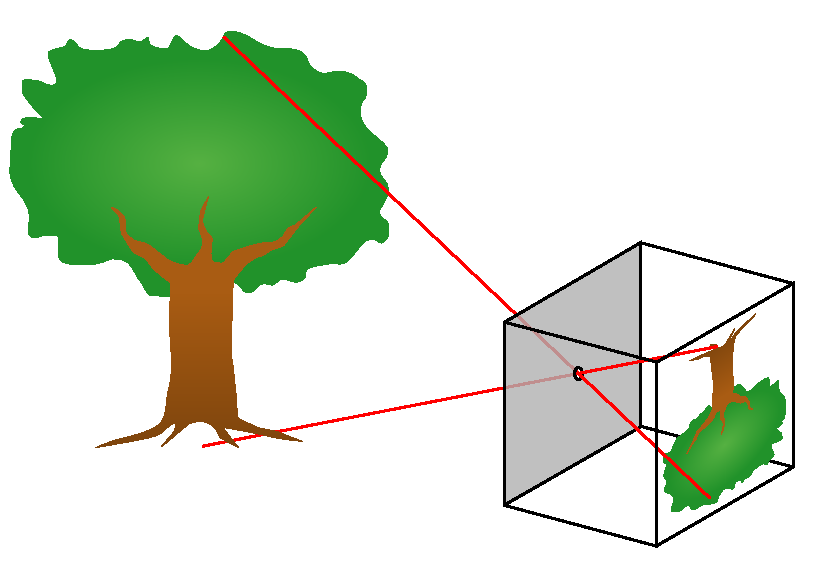
\includegraphics[width=0.5\linewidth]{imgs/pinhole.pdf}
    \caption{In this homework, we will implement 3D rendering by projecting 3D objects onto images. This is similar to a real-world camera. In particular, we will implement an ideal \href{https://en.wikipedia.org/wiki/Pinhole_camera}{pinhole camera}. Figure taken from \href{https://commons.wikimedia.org/wiki/File:Pinhole-camera.svg}{Wikipedia}.}
    \label{fig:pinhole}
\end{figure}


To make projection easier, we will focus on representing 3D surfaces, instead of the full volume. Instead of supporting multiple shapes (circles, squares, etc) like last time, we will focus on a single primitive: triangle. A main reason is that triangle has a very cool property: after perspective projection to 2D, it's still a triangle! (See \cref{fig:perspective}.) Many other shapes do not have this nice property -- a sphere projecting on to 2D can be an ellipse, a square projecting to the screen can become a general quadrilateral.

\begin{figure}[h]
    \centering
    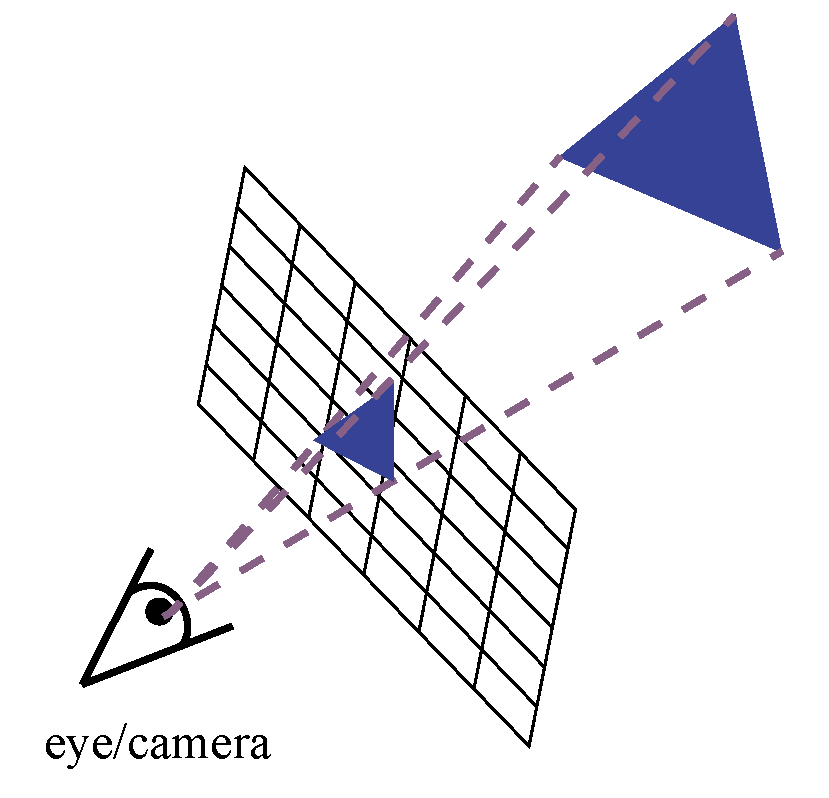
\includegraphics[width=0.5\linewidth]{imgs/perspective_projection.pdf}
    \caption{The perspective projection of a triangle.}
    \label{fig:perspective}
\end{figure}

\paragraph{Antialiasing.} In our previous homework, we asked you to do a 4x4 super-sampling antialiasing. In this homework we don't do antialiasing. Testing pixel center is good enough.

\section{Rendering a single 3D triangle (5 pts)}
\label{sec:single_triangle}

Let's start simple and render just a single 3D triangle. Our plan is to first project the triangle to a 2D image plane, then we can either use code from our previous homework, or use a more specialized \emph{edge equation test} to determine whether a point is inside a triangle. We'll discuss the edge equation test later.

\begin{figure}[h]
    \centering
    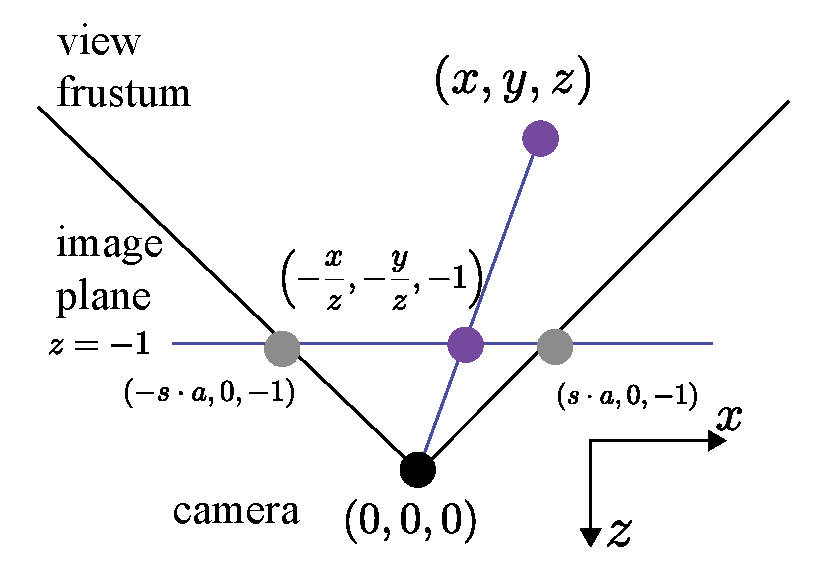
\includegraphics[width=0.5\linewidth]{imgs/perspective_transform.pdf}
    \caption{To perform perspective projection, we setup the coordinate system of the camera space so that the origin of the camera is at $(0, 0, 0)$, the camera is facing negative $z$-axis, $x$-axis is pointing right, and $y$-axis is pointing up. We put the image plane at $z=-1$. The perspective projection of a point $(x, y, z)$ is then simply finding the intersection between the line formed by the point and the camera origin with the image plane. Since our image plane has a finite extent, we further clips all point outside of $[-sa, -s, -1] \times [sa, s, -1]$ where $a$ is the aspect ratio ($\frac{\text{image width}}{\text{image height}}$) and $s$ is the scaling factor controlling the size of our image. The clipping defines a \emph{view frustum}.}
    \label{fig:perspective_transform}
\end{figure}

How do we project the triangle then? It's significantly easier if we assume a particular coordinate system of our camera. We will lift this assumption in the later part of the homework (by, you guess it, applying 3D transformations). Let's assume in the \emph{camera space}, $x$-axis is pointing right, $y$-axis is pointing up, and $z$-axis is pointing away from the direction the camera is looking at (the $z$ is specified this way so that we are following a \href{https://en.wikipedia.org/wiki/Right-hand_rule}{right-handed} coordinate system). We also assume that the image plane is located at $z=-1$ -- this is where we are going to project our triangle onto. \cref{fig:perspective_transform} shows that the perspective projection of a point $(x, y, z)$ boils down to computing the intersection between the line formed by the point and the camera origin with the image plane. The projected point $(x', y')$ is
\begin{equation}
\left(x', y'\right) = \left(-\frac{x}{z}, -\frac{y}{z}\right).
\label{eq:projection}
\end{equation}

Furthermore, we need to define the extent of the image plane (we can't have an image with infinite size!). Note that our image can be a rectangle (instead of a square). We define the extent of the image plane to be $[-sa, -s, -1] \times [sa, s, -1]$: $s$ is a scaling factor that controls the size of the image (it's half of the sensor size), and $a$ is the aspect ratio ($\frac{\text{image width}}{\text{image height}}$). $s$ is related to the vertical \href{https://en.wikipedia.org/wiki/Field_of_view}{field of view} $\alpha$ of a camera:
\begin{equation}
s = \tan\left(\frac{\alpha}{2}\right).
\end{equation}

Any pixel that lands outside of the extent of the image plane is discarded and not going to show up in our image. We call the set of points that are going to land on the image planes the \emph{view frustum}. \cref{fig:perspective_transform} also visualizes the view frustum.

\begin{figure}[h]
    \centering
    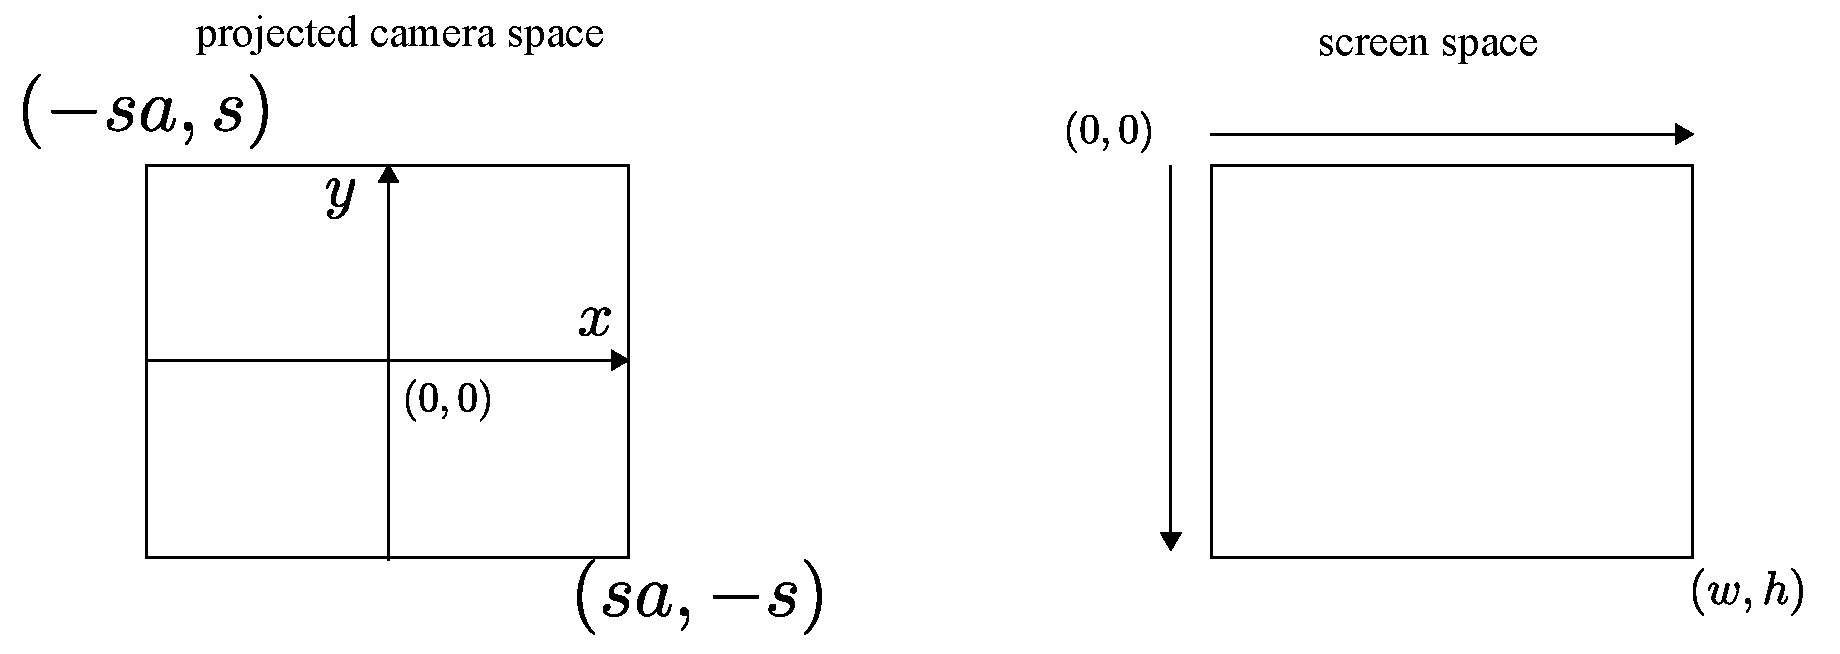
\includegraphics[width=0.9\linewidth]{imgs/camera_vs_screen.pdf}
    \caption{The different coordinate systems between our projected camera space and screen space.}
    \vspace{-20pt}
    \label{fig:camera_vs_screen}
\end{figure}

There are a few other complications though. Firstly, the point $(x', y')$ is in the projected camera space after the projection. We will need to transform it into the screen space. Recall that our screen space has $x$-axis pointing right with $y$-axis pointing down, and the extent is $[0, 0] \times [\text{width}, \text{height}]$. See \cref{fig:camera_vs_screen}. So we need to further convert the point $(x', y')$ from the projected camera space to screen space. Looking at \cref{fig:camera_vs_screen}, we can see that the we need to translate the origin, scale the axes, and flip the $y$ axis. We will give you the formula for the $x$-axis, and you should figure out the $y$-axis formula yourself:
\begin{equation}
x'' = w\frac{x'+sa}{2sa},
\label{eq:camera_to_screen}
\end{equation}
where $w$ is the width of the image.

The second complication is that a triangle vertex can be behind the camera i.e., $-z \leq 0$. In fact, even if $z$ is very close to zero, it can be still problematic: recall that in \cref{eq:projection}, we need to divide by $-z$ for the projection. When $z$ is very close to zero, the division can be unstable due to limited floating point precision. Hence, we consider all points such that $-z \leq z_{\text{near}}$ to be behind the camera. $z_{\text{near}}$ is usually called the \emph{near clipping plane}. Though, for Homework 2.1 to 2.5, we will never test you with the case with triangles having vertices behind the near clipping plane.

Dealing with triangles with only one or two vertices behind the camera, and the other in front of the camera is tricky: we will need to implement \emph{clipping}. See \cref{fig:triangle_clipping}.

\begin{figure}[h]
    \centering
    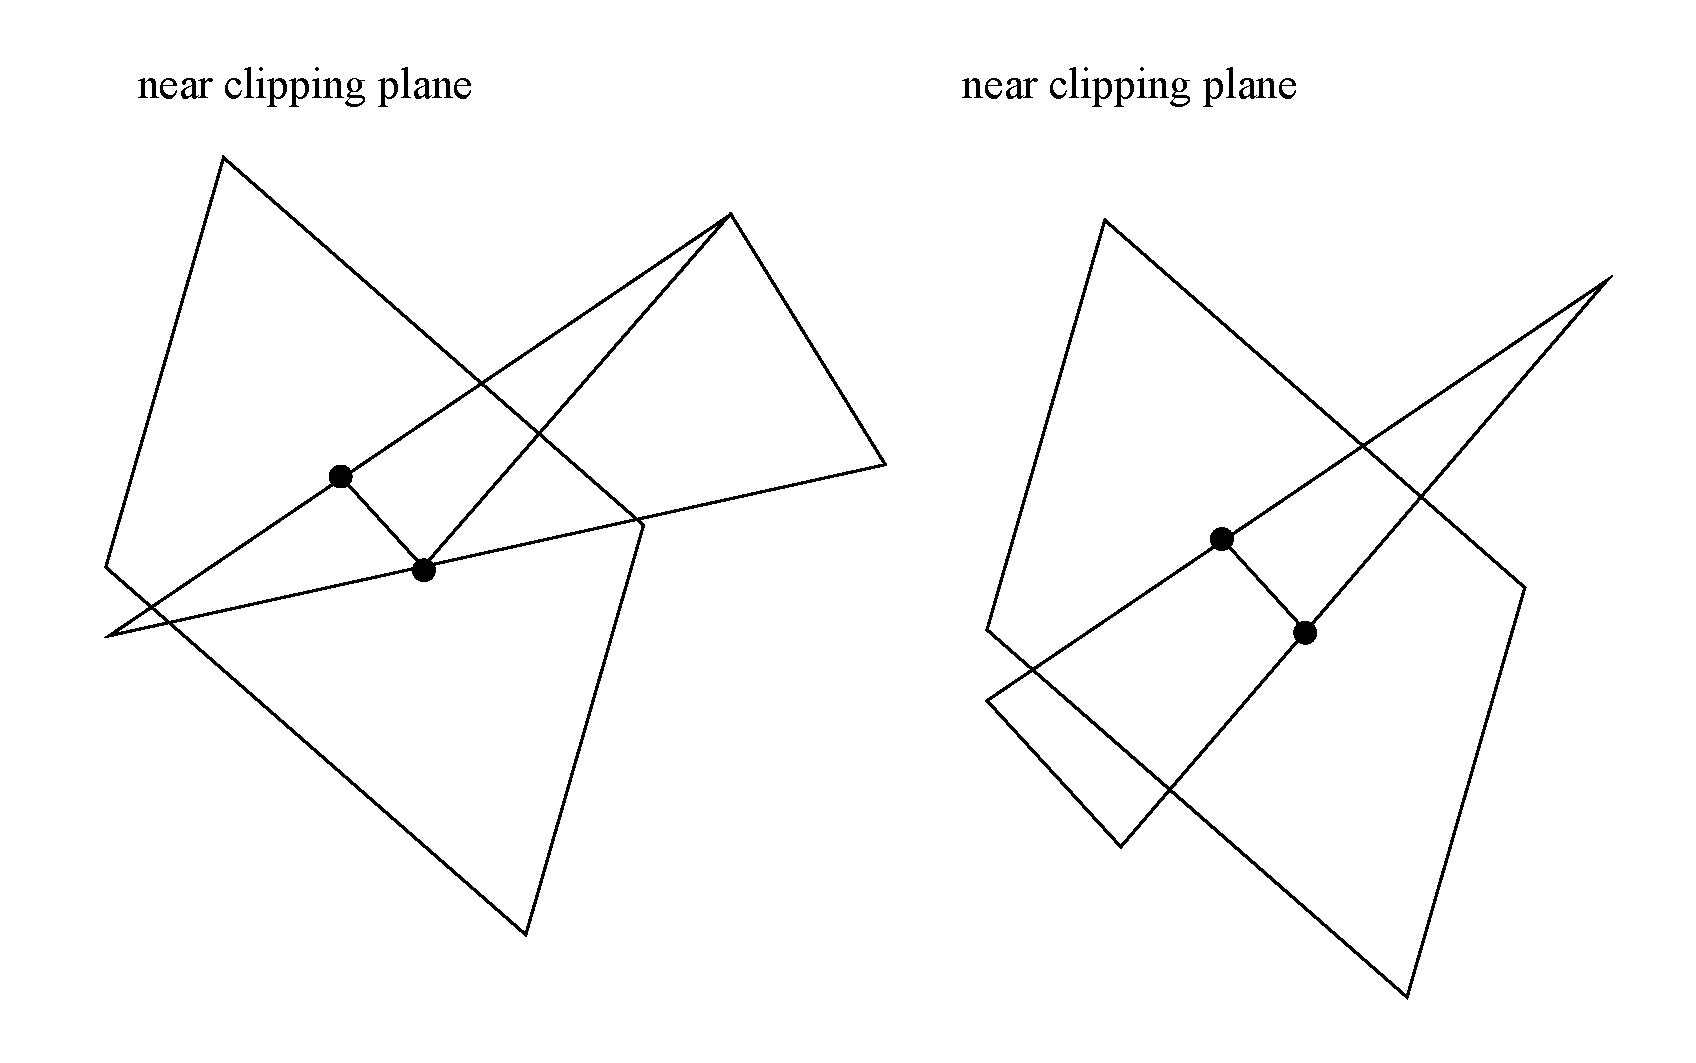
\includegraphics[width=0.7\linewidth]{imgs/triangle_clipping.pdf}
    \caption{If one or two vertices of a triangle is behind the near clipping plane, then (ideally) we would need to clip the triangle. If only one vertex is behind the clipping plane (left), then we need to clip and further split the resulting quadrilateral into two triangles. If two vertices are behind the clipping plane (right), the clipped triangle is still a triangle.}
    \label{fig:triangle_clipping}
\end{figure}

\paragraph{Mapping the computation to GPU.} We will implement one small acceleration that will be helpful later. Instead of launching one thread per pixel for the entire image, we first clear the image into its background color, and only launch thread inside the 2D \emph{Axis-Aligned Bounding Box} (AABB) of the triangle after it is projected to the screen space. See \cref{fig:aabb} for an illustration of the AABB of a 2D triangle. We have given you the rendering loop, it looks like
\begin{lstlisting}[language=Python]
# Clear the image to background color
command_encoder.clear_texture_float(img, clear_value=spy.float4(0.5, 0.5, 0.5, 1.0))
vars = {'sp0': sp0,
        'sp1': sp1,
        'sp2': sp2,
        'aabb_min': aabb_min,
        'color': args.color}
# Launch the kernel 
compute_shader.kernel.dispatch(
    thread_count=[aabb_max[0] - aabb_min[0] + 1,
                  aabb_max[1] - aabb_min[1] + 1,
                  1],
    command_encoder=command_encoder,
    image=img,
    **vars,
)
\end{lstlisting}
See \lstinline{hw2/hw2.py} for details.

Your jobs are 1) compute the screen space position of the triangle \lstinline{sp0, sp1} and \lstinline{sp2} in Python, 2) compute the AABBs, represented by the integer minimal and maximal X-Y positions on screen space (\lstinline{aabb_min} and \lstinline{aabb_max}), and 3) fill in the compute shader in \lstinline{hw2/hw2_1.slang} to actually fill out the color.

\paragraph{Edge equations.} You are welcome to use your Homework 1 code for testing whether the pixel center is inside a triangle or not, but it can be fairly inefficient and unnecessarily complex. Instead, we can use \emph{edge equations} to test whether a point is inside a triangle. The idea is that the three edges of the triangle each split the 2D domain into two half-planes. We can use dot products to test whether a point is on the positive half-plane or negative half-plane of an edge. If a point is on the positive half-planes of all three edges at the same time, or it's on the negative half-planes of all three edges at the same time, then the point is inside the triangle. More precisely, assuming the triangle has non-zero area, let the three 2D vertices be $v_0$, $v_1$, and $v_2$, and the three edges be $e_{01} = v_1 - v_0$, $e_{12} = v_2 - v_1$, and $e_{20} = v_0 - v_2$. We can compute the 2D normals of the edges as $n_{ij} = (e_{ij,y}, -e_{ij,x})$. For a 2D point $\mathbf{p}$, the edge equation is
\begin{equation}
	E_{ij}(\mathbf{p}) = (\mathbf{p} - v_i) \cdot n_{ij}.
\end{equation}
We can compute $E_{ij}(\mathbf{p})$ for the pixel center $\mathbf{p} = (x+0.5, y+0.5)$ and check its sign. If it's all nonpositive or all nonnegative, the point is inside triangle.

\begin{figure}[h]
    \centering
    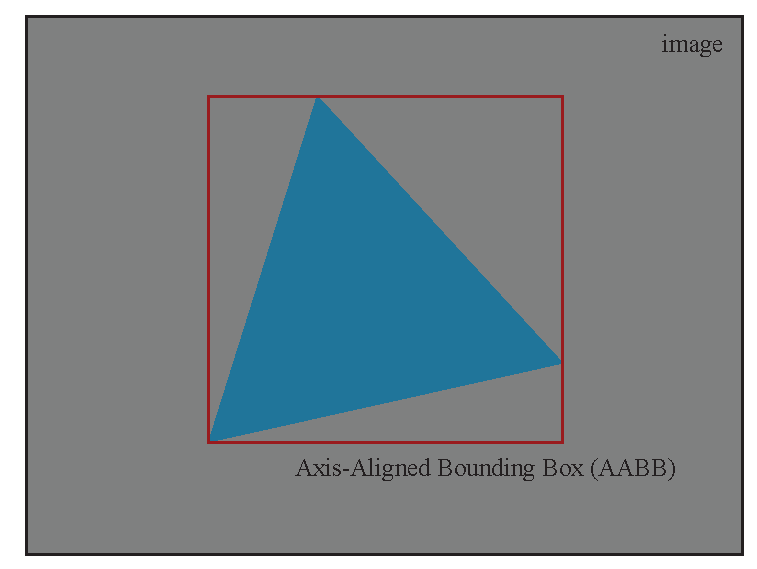
\includegraphics[width=0.7\linewidth]{imgs/aabb.pdf}
    \caption{For each triangle, we only launch threads within its Axis-Aligned Bounding Box (AABB) in the screen space. For example, if the three 2D vertices are $(123.45, 234.56), (223.45, 334.56)$, and $(23.45, 434.56)$, then the 2D AABB of this triangle has $p_{\text{min}} = (23, 234)$ and $p_{\text{max}} = (224, 435)$.}
    \label{fig:aabb}
\end{figure}

Implement your triangle rendering in \lstinline{hw2_1()} in \lstinline{hw2/hw2.py} and \lstinline{compute_main()} in \lstinline{hw2/hw2_1.slang}. To test your rendering, use the following commands:
\begin{lstlisting}[language=bash]
	uv run python main.py 2_1 -s 1 -p0 -1 -1 -3 -p1 0 1 -3 -p2 1 -1 -3 -color 0.7 0.3 0.4
	uv run python main.py 2_1 -s 0.5 -p0 -1 0 -2 -p1 0 2 -4 -p2 1 -2 -5 -color 0.7 0.3 0.8
	uv run python main.py 2_1 -s 1.5 -p0 2 2 -1 -p1 -1 -1 -2 -p2 2 0 -3 -color 0.3 0.8 0.2
	uv run python main.py 2_1 -s 1 -p0 200 200 -100 -p1 1 3 -4 -p2 -2 -2 -2 -color 0.8 0.1 0.3
\end{lstlisting}
or just any parameters you like! 

We provide our rendering of the first command in \cref{fig:hw2_1}.
\begin{figure}[h]
    \centering
    
\includegraphics[width=0.5\linewidth]{imgs/hw_2_1.png}
    \caption{Reference rendering for homework 2.1.}
    \label{fig:hw2_1}
\end{figure}

In your submission, save the image generated by the following special commands that skip the GUI:
\begin{lstlisting}[language=bash]
  uv run python main.py -output hw2_1_1.png 2_1 -s 0.5 -p0 -1 -1 -3 -p1 0 1 -3 -p2 1 -1 -3 -color 0.7 0.3 0.4
  uv run python main.py -output hw2_1_2.png 2_1 -s 1 -p0 200 200 -100 -p1 1 3 -4 -p2 -2 -2 -2 -color 0.8 0.1 0.3 
\end{lstlisting}
We will compare your output with our rendering for grading.

\section{Rendering a triangle mesh (20 pts)}
\label{sec:triangle_mesh}

\begin{figure}[h]
    \centering
    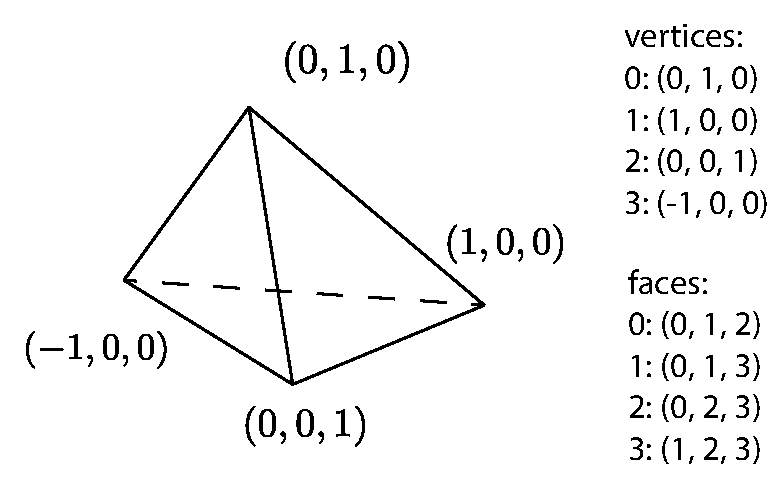
\includegraphics[width=0.7\linewidth]{imgs/triangle_mesh.pdf}
    \caption{A triangle mesh contains a list of vertices (3D positions) and a list of faces (3 integers pointing towards the index of the vertices). The figure shows a case of a triangle mesh with 4 vertices and 4 faces/triangles. The first face represents the triangle on the right side, the second face represents the triangle at the back, the third face represents the triangle on the left, and the last face represents the triangle at the bottom.}
    \label{fig:triangle_mesh}
\end{figure}

Next, we'll extend our previous code to handle more than one triangle. In computer graphics, we often store these triangles in a data structure called ``triangle mesh'' (\cref{fig:triangle_mesh}). Additionally, to visualize the mesh, we store RGB color at each mesh vertex. Triangle mesh is a more efficient data structure than simply storing a list of triangles since many of the triangles would share vertices in graphics (really? when will it be better and when will it not be better?). To render triangle meshes, you need to go through the face array and loop through all the triangles.

\begin{figure}[h]
    \centering
    
\includegraphics[width=0.4\linewidth]{imgs/cyclic.pdf}
    
\includegraphics[width=0.4\linewidth]{imgs/interpenetration.pdf}
    \caption{We cannot globally sort all objects into a single order by depth. The objects can form a cyclic order (left) or they can have interpenetration (right).}
    \label{fig:depth_order}
\end{figure}

An important difference, compared to the list of triangles we have in Homework 1, is to determine the depth order between all these triangles. That is, for a point inside a pixel, we need to decide which triangle is the one we actually see. The tricky part is, unlike Homework 1, it is not always possible to globally sort the triangles to determine a depth order (\cref{fig:depth_order}).

Therefore, we need to know the depth value of all the triangles overlapping with the point in the pixel. That is, given a screen space point inside a projected triangle, we need to \emph{interpolate} from the depth values of the three vertices. This turns out to be slightly involved mathematically (code-wise it's actually not that much though, my implementation of the depth interpolation takes around 60 lines including lots of comments). 

To explain how to find the desired depth value, we need to explain what are \href{https://en.wikipedia.org/wiki/Barycentric_coordinate_system}{barycentric coordinates}. Any point $\mathbf{p}$ inside a triangle with three vertices $\mathbf{p}_0$, $\mathbf{p}_1$, $\mathbf{p}_2$ can be expressed using linear combination of the three vertices:
\begin{equation}
\mathbf{p} = b_0 \mathbf{p}_0 + b_1 \mathbf{p}_1 + b_2 \mathbf{p}_2,
\end{equation}
where $b_0 + b_1 + b_2 = 1$, $b_0 \geq 0$, $b_1 \geq 0$, and $b_2 \geq 0$. Given a point $\mathbf{p}$, we can compute the \textbf{unique} coefficients using \href{https://en.wikipedia.org/wiki/Cramer%27s_rule}{Cramer's rule}:
\begin{equation}
\begin{aligned}
b_0 &= \frac{\text{area}\left(\mathbf{p}, \mathbf{p}_1, \mathbf{p}_2\right)}{\text{area}\left(\mathbf{p}_0, \mathbf{p}_1, \mathbf{p}_2\right)} \\
b_1 &= \frac{\text{area}\left(\mathbf{p}_0, \mathbf{p}, \mathbf{p}_2\right)}{\text{area}\left(\mathbf{p}_0, \mathbf{p}_1, \mathbf{p}_2\right)} \\
b_2 &= \frac{\text{area}\left(\mathbf{p}_0, \mathbf{p}_1, \mathbf{p}\right)}{\text{area}\left(\mathbf{p}_0, \mathbf{p}_1, \mathbf{p}_2\right)}
\end{aligned}
\label{eq:barycentric_solve}
\end{equation}

To get the area of a triangle, you can use the length of the cross product between two of the edge vectors, which will give you the area of the parallelogram, you can then divide the parallelogram area by two. This works also for 2D triangles, you only need to pretend the 2D triangle is on a 3D plane (e.g., $z=0$).

\begin{figure}[h]
    \centering
    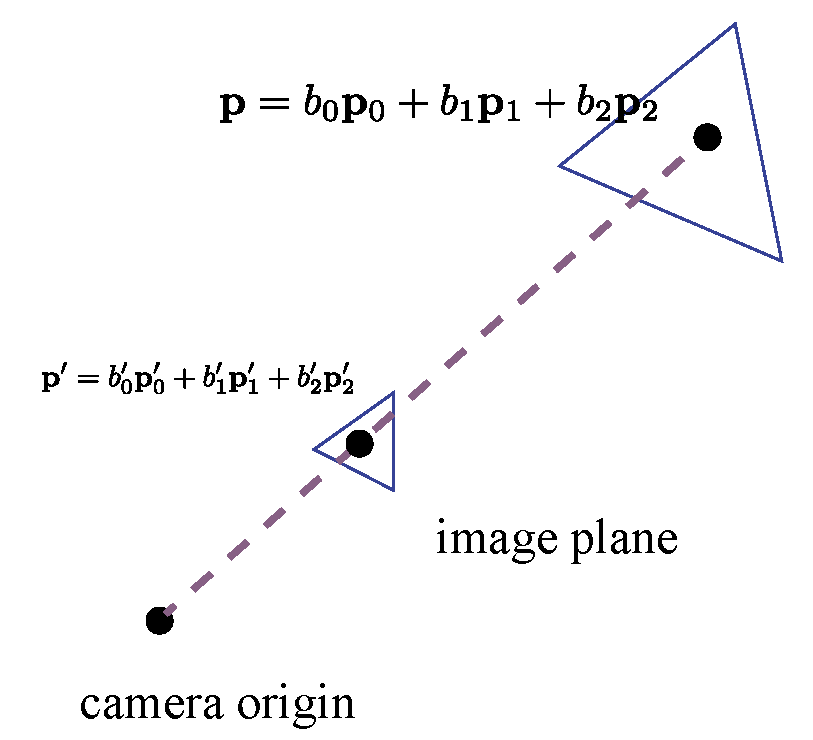
\includegraphics[width=0.5\linewidth]{imgs/perspective_interpolate.pdf}
    \caption{Given a point on image plane $p$', and a triangle with three vertices $\mathbf{p}_0$, $\mathbf{p}_1$, $\mathbf{p}_2$, we want to know the depth, i.e., the $-z$ coordinate at the corresponding point $\mathbf{p}$.}
    \label{fig:perspective_interpolate}
\end{figure}

As illustrated in \cref{fig:perspective_interpolate}, our goal is, given an image plane point $\mathbf{p}'$ and a triangle with three vertices $\mathbf{p}_0$, $\mathbf{p}_1$, and $\mathbf{p}_2$, figure out the $z$ coordinate of the corresponding point $\mathbf{p}$. We want to use barycentric coordinates to help us. So we need to figure out what $b_0$, $b_1$, and $b_2$ are, so that we can interpolate the $z$ coordinates from $\mathbf{p}_0$, $\mathbf{p}_1$, and $\mathbf{p}_2$. Unfortunately, we cannot directly use \cref{eq:barycentric_solve}, since we don't know $\mathbf{p}$ (otherwise we would have known the answer already!). 

What we do know are the original vertices $\mathbf{p}_0$, $\mathbf{p}_1$, and $\mathbf{p}_2$, projected vertices $\mathbf{p}_0'$, $\mathbf{p}_1'$, and $\mathbf{p}_2'$, and our image plane point $\mathbf{p}'$. Furthermore, we know that $\mathbf{p}$ projects to $\mathbf{p}'$ and $\mathbf{p}_i$ projects to $\mathbf{p}_i'$. Given the projected vertices and the image plane point, we can compute the projected barycentric coordinates $b_0'$, $b_1'$, $b_2'$ using \cref{eq:barycentric_solve}. We want to relate the projected barycentric coordinates with the original ones.

Since $\mathbf{p}$ projects to $\mathbf{p}'$ (which we now write as $\mathbf{p}'=(x',y',-1)$), we know that
\begin{equation}
\mathbf{p}' = \left(-\frac{\mathbf{p}.x}{\mathbf{p}.z}, -\frac{\mathbf{p}.y}{\mathbf{p}.z}, -1\right) 
= -\frac{\mathbf{p}}{\mathbf{p}.z}.
\end{equation}
(We use $\mathbf{p}.z$ to denote the z coordinate of point $\mathbf{p}$.)

Plugging in $\mathbf{p} = b_0 \mathbf{p}_0 + b_1 \mathbf{p}_1 + b_2 \mathbf{p}_2$ and $\mathbf{p}.z = b_0 \mathbf{p}_0.z + b_1 \mathbf{p}_1.z + b_2 \mathbf{p}_2.z$:
\begin{equation}
\mathbf{p}' = -\frac{b_0 \mathbf{p}_0 + b_1 \mathbf{p}_1 + b_2 \mathbf{p}_2}{b_0 \mathbf{p}_0.z + b_1 \mathbf{p}_1.z + b_2 \mathbf{p}_2.z}.
\end{equation}

Next, we know that $\mathbf{p}_0$ projects to $\mathbf{p}_0'$, $\mathbf{p}_1$ projects to $\mathbf{p}_1'$, and $\mathbf{p}_2$ projects to $\mathbf{p}_2'$:
\begin{equation}
\begin{aligned}
-\left(\mathbf{p}_0.z\right) \left(\mathbf{p}_0'\right) &= \mathbf{p}_0 \\
-\left(\mathbf{p}_1.z\right) \left(\mathbf{p}_1'\right) &= \mathbf{p}_1 \\
-\left(\mathbf{p}_2.z\right) \left(\mathbf{p}_2'\right) &= \mathbf{p}_2.
\end{aligned}
\end{equation}

Plugging in, we get
\begin{equation}
\mathbf{p}' = \frac{b_0 \left(\mathbf{p}_0.z\right) \mathbf{p}_0' + b_1 \left(\mathbf{p}_1.z\right) \mathbf{p}_1' + b_2 \left(\mathbf{p}_2.z\right) \mathbf{p}_2'}{b_0 \mathbf{p}_0.z + b_1 \mathbf{p}_1.z + b_2 \mathbf{p}_2.z}.
\end{equation}

Compare the above with:
\begin{equation}
\mathbf{p}' = b_0' \mathbf{p}_0' + b_1' \mathbf{p}_1' + b_2' \mathbf{p}_2',
\end{equation}
using the uniqueness of barycentric coordinates, we have:
\begin{equation}
\begin{aligned}
b_0' &= \frac{b_0 \mathbf{p}_0.z}{b_0 \mathbf{p}_0.z + b_1 \mathbf{p}_1.z + b_2 \mathbf{p}_2.z} \\
b_1' &= \frac{b_1 \mathbf{p}_1.z}{b_0 \mathbf{p}_0.z + b_1 \mathbf{p}_1.z + b_2 \mathbf{p}_2.z} \\
b_2' &= \frac{b_2 \mathbf{p}_2.z}{b_0 \mathbf{p}_0.z + b_1 \mathbf{p}_1.z + b_2 \mathbf{p}_2.z}.
\end{aligned}
\label{eq:projected_barycentric}
\end{equation}

We are almost there: we now want to express $b_0$, $b_1$, and $b_2$ using $b_0'$, $b_1'$, and $b_2'$. Let $B = b_0 \mathbf{p}_0.z + b_1 \mathbf{p}_1.z + b_2 \mathbf{p}_2.z$, we have:
\begin{equation}
\begin{aligned}
b_0 &= \frac{b_0' B}{\mathbf{p}_0.z} \\
b_1 &= \frac{b_1' B}{\mathbf{p}_1.z} \\
b_2 &= \frac{b_2' B}{\mathbf{p}_2.z}
\end{aligned}
\end{equation}

Furthermore, we know that $b_0 + b_1 + b_2 = 1$, so:
\begin{equation}
B = \frac{1}{\frac{b_0'}{\mathbf{p}_0.z} + \frac{b_1'}{\mathbf{p}_1.z} + \frac{b_2'}{\mathbf{p}_2.z}}.
\end{equation}

Rewriting \cref{eq:projected_barycentric} using the equation above, we have:
\begin{equation}
\begin{aligned}
\frac{\frac{b_0'}{\mathbf{p}_0.z}}{\frac{b_0'}{\mathbf{p}_0.z} + \frac{b_1'}{\mathbf{p}_1.z} + \frac{b_2'}{\mathbf{p}_2.z}} &= b_0 \\
\frac{\frac{b_1'}{\mathbf{p}_1.z}}{\frac{b_0'}{\mathbf{p}_0.z} + \frac{b_1'}{\mathbf{p}_1.z} + \frac{b_2'}{\mathbf{p}_2.z}} &= b_1 \\
\frac{\frac{b_2'}{\mathbf{p}_2.z}}{\frac{b_0'}{\mathbf{p}_0.z} + \frac{b_1'}{\mathbf{p}_1.z} + \frac{b_2'}{\mathbf{p}_2.z}} &= b_2
\end{aligned}.
\label{eq:inverse_depth_weighting}
\end{equation}
The equation above has an intuitive meaning: \textbf{the original barycentric coordinates can be obtained by the projected barycentric coordinate weighted by inverse depth}. We will use these equations again later in the homework.

Having the barycentric coordinates, we can finally get the desired Z value:
\begin{equation}
\mathbf{p}.z = b_0 \mathbf{p}_0.z + b_1 \mathbf{p}_1.z + b_2 \mathbf{p}_2.z.
\label{eq:interpolated_depth}
\end{equation}
Note that in our coordinate system, a visible triangle will have $z < 0$. For depth we want it do be positive so we set depth $d = -\mathbf{p}.z$.

To visualize the mesh, we store a color at each triangle vertex. Let the three color of a triangle be $\mathbf{c}_0, \mathbf{c}_1$ and $\mathbf{c}_2$, we again interpolate it using the barycentric coordinates:
\begin{equation}
\mathbf{c} = b_0 \mathbf{c}_0 + b_1 \mathbf{c}_1 + b_2 \mathbf{c}_2.
\label{eq:interpolated_color}
\end{equation}
By the way, this is what people mean if they say they are doing \emph{perspective-corrected interpolation} in a renderer. In contrast, the ``incorrect'' interpolation would use the 2D barycentric coordinates over the correct 3D ones.

To compare between depths of different triangles hitting the same pixel center, we store a \emph{depth image}. Each pixel of the depth image stores the current closest depth, and the depth is initialized to infinity at the beginning. 

To summarize, given an image plane point (e.g., pixel or subpixel center) and a triangle, we do the following:
\vspace{30pt}
\begin{enumerate}
    \item We first project triangle vertices to screen space using
    \cref{eq:camera_to_screen}, recall \cref{fig:camera_vs_screen}.

    \item We compute the AABB of the 2D triangle, and launch a GPU
    kernel for each triangle. For each kernel we have one thread
    per pixel inside the AABB.

    \item For each GPU thread, if the corresponding image plane
    pixel center is inside the triangle, we do the following:
    \begin{enumerate}
        \item We convert the current image plane point from screen
        space to the projected camera space.

        \item We compute the projected barycentric coordinates
        $b_0'$, $b_1'$, and $b_2'$ using
        \cref{eq:barycentric_solve}.

        \item Using the projected barycentric coordinates and the
        depth at the three vertices, we convert them to the original
        barycentric coordinates using \cref{eq:inverse_depth_weighting}.

        \item We obtain the Z values/depth using
        \cref{eq:interpolated_depth}, compare the depth with the
        depth image at the same pixel, and update the depth if
        the new depth is smaller.

        \item If the new depth is indeed smaller, update the color
        image using barycentric coordinates interpolated vertex
        color (\cref{eq:interpolated_color}).
    \end{enumerate}
\end{enumerate}

Now you should be ready to implement the rendering of a triangle mesh! You'll need to fill in some Python code in \lstinline{hw2_2()} and some Slang code in \lstinline{hw2_2.slang}. Test your implementation using
\begin{lstlisting}[language=bash]
  uv run python main.py 2_2 -s 1.0 scenes/hw2/two_shapes_mesh.json
  uv run python main.py 2_2 -s 0.6 scenes/hw2/cube_mesh.json
\end{lstlisting}

Our rendering for \lstinline{two_shapes_mesh.json} is in \cref{fig:hw2_2}.
\begin{figure}[h]
    \centering
    
\includegraphics[width=0.5\linewidth]{imgs/hw_2_2.png}
    \caption{Reference rendering for homework 2.2.}
    \label{fig:hw2_2}
\end{figure}

To test your code, we will use these commands:
\begin{lstlisting}[language=bash]
  uv run python main.py -output outputs/hw_2_2_1.png 2_2 -s 0.6 scenes/hw2/quad_mesh.json
  uv run python main.py -output outputs/hw_2_2_2.png 2_2 -s 1.1 scenes/hw2/depth_layers_mesh.json
  uv run python main.py -output outputs/hw_2_2_3.png 2_2 -s 0.5 scenes/hw2/torus_mobius_mesh.json
\end{lstlisting}
We will compare your renderings with ours.

This part is more involved than the previous part. A way to debug is to render the same triangle as in \cref{sec:single_triangle} using your \cref{sec:triangle_mesh} code -- if they are different, then something is wrong and you can check what led to that problem.

Due to floating point precision, your implementation may occasionally produce small cracks along shared triangle edges. You do not need to handle these cases in this homework. Real rasterizers handle this using fixed-point math and very carefully designed fill rule. See \href{https://fgiesen.wordpress.com/2013/02/08/triangle-rasterization-in-practice/}{this blog post} from Fabian Giesen for more explanation.

\section{3D transformation (20 pts)}

So far we have assumed that everything is in the camera space and camera is always located at $(0, 0, 0)$ facing negative $z$ with up vector $y$. Let's add some transformations so that things are less restricted. Remember that in the 2D case in Homework 1, we use a $3 \times 3$ matrix to represent affine transformations. Here, we will use a $4 \times 4$ matrix. Like in 2D, we will support scaling, translation, and rotation (shearing is also possible, but we want to save you some typing). Furthermore, we will support two kinds of new transformations: lookAt transform and perspective transform that we will talk about soon. 

\begin{figure}[h]
    \centering
    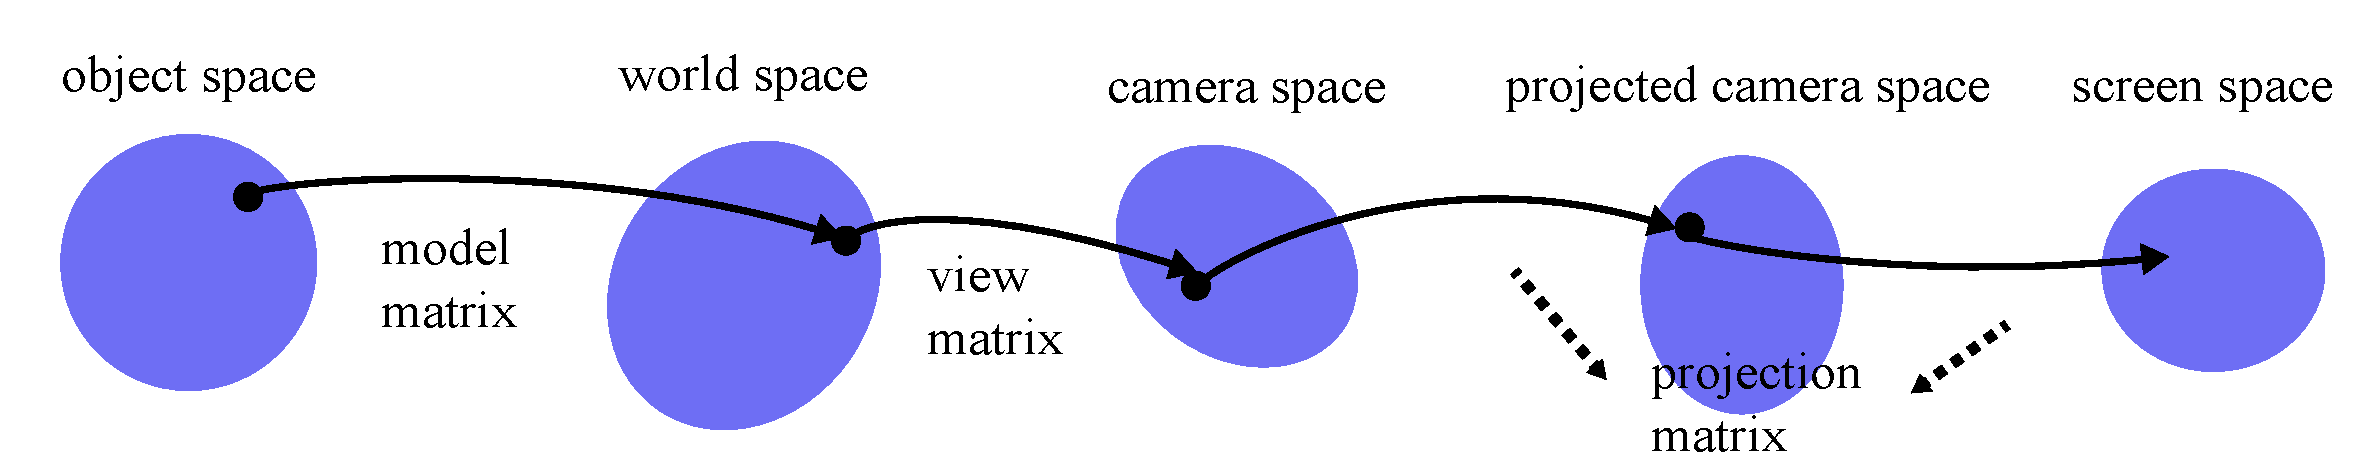
\includegraphics[width=0.8\linewidth]{imgs/3d_spaces.pdf}
    \caption{Spaces and the transformations between them in 3D.}
    \label{fig:3d_spaces}
\end{figure}

Before we explain the 3D transformations, we need to explain our spaces in 3D. Previously in 2D, we only had \emph{object space} and \emph{canvas space}. The existence of the camera makes things slightly more complicated: the camera lives in the \emph{camera space} (the coordinate system in the previous parts), and the matrices now transform the objects into \emph{world space}. As a convention, we usually call the object-to-world transformation the \emph{model matrix} $M$, the world-to-camera transformation the \emph{view matrix} $V$, the camera-to-screen transformation the \emph{projection matrix} $P$ (yes, we can express the projection as a matrix! more on this later). Given a vertex $v$ on a 3D triangle mesh, we can chain the transformations to project it onto the screen space: $v'=PVMv$ (unfortunately, the combined matrix $PVM$ is usually called the ``MVP'' matrix). \cref{fig:3d_spaces} illustrates this. Note that the last two steps are what we did in \cref{sec:triangle_mesh}, where we project the triangles from camera space to projected camera space, and then to the screen space. 

\paragraph{Scaling and translation.} Scaling and translations are basically the same as in 2D:
\begin{equation}
\begin{bmatrix}
x' \\
y' \\
z' \\
1
\end{bmatrix}
=
\begin{bmatrix}
s_x & 0 & 0 & 0 \\
0 & s_y & 0 & 0 \\
0 & 0 & s_z & 0 \\
0 & 0 & 0 & 1
\end{bmatrix}
\begin{bmatrix}
x \\
y \\
z \\
1
\end{bmatrix}
\end{equation}

\begin{equation}
\begin{bmatrix}
x' \\
y' \\
z' \\
1
\end{bmatrix}
=
\begin{bmatrix}
1 & 0 & 0 & t_x \\
0 & 1 & 0 & t_y \\
0 & 0 & 1 & t_z \\
0 & 0 & 0 & 1
\end{bmatrix}
\begin{bmatrix}
x \\
y \\
z \\
1
\end{bmatrix}
\end{equation}

\paragraph{Rotation.} Rotation in 3D is a lot more complicated. Unlike 2D, which we pretty much only have two ways to rotate (clockwise or counterclockwise), in 3D there are infinitely many ways to rotate. We will (hopefully) talk about a lot of them in the lectures towards the end of the quarter, but for this homework we will implement a simple rotation mechanism called Euler angles. That is, we describe rotation only over $x, y$, and $z$ axes, thus reducing 3D rotations into 3 2D rotations.

\begin{align}
R_x(\theta) &=
\begin{pmatrix}
1 & 0 & 0 & 0 \\
0 & \cos\theta & -\sin\theta & 0 \\
0 & \sin\theta & \cos\theta & 0 \\
0 & 0 & 0 & 1
\end{pmatrix}, \\[1em]
R_y(\theta) &=
\begin{pmatrix}
\cos\theta & 0 & \sin\theta & 0 \\
0 & 1 & 0 & 0 \\
-\sin\theta & 0 & \cos\theta & 0 \\
0 & 0 & 0 & 1
\end{pmatrix}, \\[1em]
R_z(\theta) &=
\begin{pmatrix}
\cos\theta & -\sin\theta & 0 & 0 \\
\sin\theta & \cos\theta & 0 & 0 \\
0 & 0 & 1 & 0 \\
0 & 0 & 0 & 1
\end{pmatrix}.
\end{align}

Because 3D rotations do not commute (which is one reason why they are so annoying), Euler angles rotation typically compose these three matrices in a particular order like $R_z(\theta_z) R_y(\theta_y) R_x(\theta_x)$. In our homework, we simply allow the users to use \lstinline{rotate_x}, \lstinline{rotate_y}, and \lstinline{rotate_z} inside their transformations.

\begin{figure}[h]
    \centering
    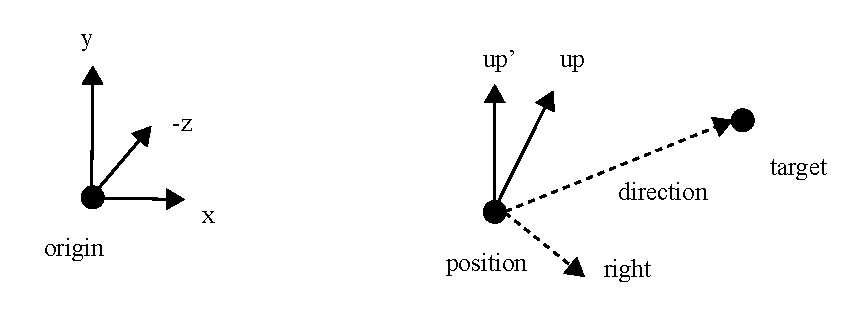
\includegraphics[width=0.7\linewidth]{imgs/lookat.pdf}
    \caption{The LookAt transform maps a coordinate frame based on the parameters \lstinline{position}, \lstinline{target}, and \lstinline{up}. $-z$ axis is mapped to the \lstinline{direction} of \lstinline{target - position}, $x$ axis is mapped to the cross product of \lstinline{direction} and \lstinline{up}, and $y$ axis is mapped to the cross product of \lstinline{right} and \lstinline{direction}.}
    \label{fig:lookat}
\end{figure}

\paragraph{LookAt.} The LookAt transform is useful for positioning cameras. The LookAt transform takes 2 3D points and a 3D vector as parameters: the \lstinline{position} of the object $\mathbf{p}$, the \lstinline{target} the object is looking at $\mathbf{t}$, and the \lstinline{up} vector $\mathbf{u}$ that describe the orientation of the object. \cref{fig:lookat} illustrates the geometry.

Given the input, we first compute where the camera should be facing using $\mathbf{p}$ and $\mathbf{t}$:
\begin{equation}
\mathbf{d} = \text{normalize}(t - p).
\end{equation} 
Given the \lstinline{direction} $\mathbf{d}$, we can then compute the \lstinline{right} vector $\mathbf{r}$ using cross product with the given \lstinline{up} vector $\mathbf{u}$:
\begin{equation}
\mathbf{r} = \text{normalize}\left(\mathbf{d} \times \mathbf{u}\right).
\end{equation}

We are not done yet though. Since the up vector $\mathbf{u}$ is not necessarily perpendicular to the camera direction $\mathbf{d}$, we do not have an orthonormal basis yet. Thus we recompute the up vector using the cross product between the right vector and the camera direction:
\begin{equation}
\mathbf{u}' = \mathbf{r} \times \mathbf{d}.
\end{equation}

Given this information, we can build our transformation matrix:
\begin{equation}
L = 
\begin{bmatrix}
\mathbf{r}.x & \mathbf{u}'.x & -\mathbf{d}.x & \mathbf{p}.x \\
\mathbf{r}.y & \mathbf{u}'.y & -\mathbf{d}.y & \mathbf{p}.y \\
\mathbf{r}.z & \mathbf{u}'.z & -\mathbf{d}.z & \mathbf{p}.z \\
0 & 0 & 0 & 1 
\end{bmatrix}
\end{equation}

The first column sends $x$ axis ($(1, 0, 0)$) to $\mathbf{r}$, the second column sends $y$ axis ($(0, 1, 0)$) to $\mathbf{u}'$, the third column sends $z$ axis to $-\mathbf{d}$, and the last column translates the coordinate systems by $\mathbf{p}$.

Note that when applied to cameras, the matrix $L$ is designed to transform from camera space to world space. When constructing the view matrix (\cref{fig:3d_spaces}), we need to go from world space to the camera space. 

\paragraph{Perspective projection.}
Now we are at the coolest part. It turns out that with some math tricks, we can turn the perspective projection we did in the first part (\cref{fig:perspective_transform}) into a matrix multiplication as well! The trick is to introduce something called the \href{https://en.wikipedia.org/wiki/Homogeneous_coordinates}{homogeneous coordinates}. The idea is to make use of the 4th component of the vector. So far, we always assumed that the 4th component to be either $1$ or $0$ (when it's $0$, it's a vector instead of a point). From now on, our vectors can have arbitrary 4th component:
\begin{equation}
\begin{bmatrix}
x \\
y \\
z \\
w
\end{bmatrix}.
\end{equation}
The clever part is how we obtain the 3D vector from the 4D vector above: we define everything to be equivalent up to an arbitrary non-zero scaling:
\begin{equation}
\begin{bmatrix}
x \\
y \\
z \\
w
\end{bmatrix} \sim
\begin{bmatrix}
\frac{x}{w} \\
\frac{y}{w} \\
\frac{z}{w} \\
1
\end{bmatrix}.
\end{equation}

Following this definition, we can implement \cref{eq:projection} using the following matrix multiplication:
\begin{equation}
\begin{bmatrix}
x' \\
y' \\
z' \\
w'
\end{bmatrix} =
\begin{bmatrix}
1 & 0 & 0 & 0 \\
0 & 1 & 0 & 0 \\
0 & 0 & 0 & 1 \\
0 & 0 & -1 & 0
\end{bmatrix}
\begin{bmatrix}
x \\
y \\
z \\
1
\end{bmatrix}.
\end{equation}
Notice that all four components are computed using linear operations. The nonlinear perspective projection only shows up after we divide by the fourth component.
\begin{equation}
\begin{bmatrix}
x' \\
y' \\
z' \\
w'
\end{bmatrix}
=
\begin{bmatrix}
x \\
y \\
1 \\
-z
\end{bmatrix}
\sim
\begin{bmatrix}
-\frac{x}{z} \\
-\frac{y}{z} \\
-\frac{1}{z} \\
1
\end{bmatrix}.
\end{equation}
A bonus we get is that after the homogeneous division, the third component becomes the reciprocal depth $-\frac{1}{z}$: we can directly use it for getting the barycentric coordinates (\cref{eq:inverse_depth_weighting})!

Remember that the projection above only projects within the camera space. We need to further convert to screen space (\cref{eq:camera_to_screen}). I'll let you figure out how the matrix should look like! 

Now you should have everything you need to complete this homework. 

Like Homework 1, we will describe the camera transformation and the meshes in a JSON scene file. 

A scene file would look like this:

\begin{lstlisting}[language=json]
{
    "camera":
    {
        "resolution": [640, 480],
        "transform": [
            {
                "lookat":
                {
                    "position": [0, 1, 0],
                    "target": [0, 0, -5],
                    "up": [0, 1, 0]
                }
            }
        ],
        "s": 1
    },
    "background": [
        0.5, 0.5, 0.5
    ],
    "objects": [
        {
            "filename": "two_shapes_mesh.json",
            "transform": [
                {"rotate_x": [10]},
                {"scale": [0.9, 1.1, 0.8]},
                {"translate": [-0.2, -0.2, 0.2]}
            ]
        }
    ]
}
\end{lstlisting}

In our scene files, transformations are applied in the order they are listed. For example, a rotation followed by a translation corresponds to $TR$, not $RT$.

Instead of directly specifying the vertices/faces in a JSON file, we can also use the \href{https://en.wikipedia.org/wiki/PLY_(file_format)}{Stanford PLY format}:
\begin{lstlisting}[language=json]
{
    "camera":
    {
        "resolution": [640, 480],
        "transform": [
            {
                "lookat":
                {
                    "position": [1, 1, 0],
                    "target": [0, 0, -5],
                    "up": [0, 1, 0]
                }
            }
        ],
        "s": 1
    },
    "background": [
        0.5, 0.5, 0.5
    ],
    "objects": [
        {
            "filename": "tetrahedron.ply",
            "transform": [
                {"scale": [1.5, 0.8, 0.7]},
                {"translate": [0.5, -0.3, 0.2]}
            ]
        }
    ]
}
\end{lstlisting}
The PLY file is human readable (when in the ``ascii'' mode) and looks like this:
\begin{lstlisting}
ply
format ascii 1.0
comment Created by Blender 3.4.1 - www.blender.org
element vertex 4
property float x
property float y
property float z
property float red
property float green
property float blue
element face 4
property list uchar uint vertex_indices
end_header
-0.483444 0.826069 -2.307457 0.75 0.35 0.35
1.152029 -1.111880 -1.928058 0.35 0.75 0.35
1.485437 0.880605 -2.239198 0.35 0.35 0.75
0.594299 0.143237 -1.466344 0.75 0.35 0.75
3 0 1 2
3 1 3 2
3 3 1 0
3 2 3 0
\end{lstlisting}

Like in Homework 1, your first task is to implement the transformations in \lstinline{compose_transformations} in \lstinline{hw2/hw2_scene.py}. Next, you'll render the parsed scene in \lstinline{hw2_3} in \lstinline{hw2/hw2.py}. We will use the same compute shader as 2.2, so everything you need to do for this part is in Python.

Note that our camera data structure stores the matrix \lstinline{cam_to_world}. The ``view matrix'' in \cref{fig:3d_spaces} is the inverse of \lstinline{cam_to_world}.

To test your rendering, use the following commands:
\begin{lstlisting}[language=bash]
  uv run python main.py 2_3 scenes/hw2/two_shapes_scene.json
  uv run python main.py 2_3 scenes/hw2/torus_mobius_scene.json
\end{lstlisting}

To test your code, we will use these commands:
\begin{lstlisting}[language=bash]
  uv run python main.py -output outputs/hw_2_3_1.png 2_3 scenes/hw2/two_shapes_side.json
  uv run python main.py -output outputs/hw_2_3_2.png 2_3 scenes/hw2/two_shapes_order.json
  uv run python main.py -output outputs/hw_2_3_3.png 2_3 scenes/hw2/three_instances.json
\end{lstlisting}
We will compare your renderings with ours.

\section{3D Animation (15 points)}
Let's make things move! Like the previous homework, we will create animation using keyframes that interpolate transformation parameters. For rotations, an interpolation from 0 degree to 360 degree should produce a full turn. Our scene format supports animation through \lstinline{transform_keyframes}. Each keyframe specifies a time (in seconds) and a list of transformations. We assume that all keyframes have the same number and types of transformations, in the same order. We interpolate the corresponding parameters of each transformation independently. The animation repeats every duration seconds. If an object has no animation keyframes, we use its static transform, as before. Otherwise, the animated transformation replaces the static transformation. The first and last keyframes should cover the interval from $0$ to \lstinline{scene.duration}.

This part should be easier than the others. Your task is to implement \lstinline{interpolate_transformation()} in \lstinline{hw2/hw2.py} so that the camera and meshes can move over time. You can reuse your existing rasterization code and all the transformation functions from the previous parts. You can reuse almost all of your implementation from the previous part. The main difference is that the camera and model matrices now depend on time. You still do not need to modify any Slang code.

To test your rendering, use the following commands:
\begin{lstlisting}[language=bash]
  uv run python main.py 2_4 scenes/hw2/two_shapes_animation.json
  uv run python main.py 2_4 scenes/hw2/torus_mobius_animation.json
\end{lstlisting}
For the first one you should see the two shapes rotating in the y axis. For the second one you should see the torus and the Mobius strip jumping around.

To test your code, we will use these commands:
\begin{lstlisting}[language=bash]
  uv run python main.py -output outputs/hw_2_4_1.png 2_4 -time 5.0 scenes/hw2/torus_mobius_spin.json
  uv run python main.py -output outputs/hw_2_4_2.png 2_4 -time 0.6 scenes/hw2/torus_mobius_dolly.json
  uv run python main.py -output outputs/hw_2_4_3.png 2_4 -time 6.0 scenes/hw2/two_instances_animation.json
\end{lstlisting}
We will compare your renderings with ours.

\section{Accelerating parallel rasterization (15 points)}

This is probably the ``boss fight'' of this homework, similar to the Bezier curves part of the last homework. After this one things will be a lot easier.

Our previous code works fine when the triangles are large and there are only a few of them, 
but it is not very parallel because it serially launch GPU kernels for each triangle, and the barriers force us to wait for the previous kernel to finish.
Imagine a scene with a million triangles, but each only occupy one or two pixels. Our previous code will essentially serialize the entire computation
and give up the powerful parallelization provided by the GPU.

In this section we will make the rasterizer faster. Our method is inspired by a software rasterizer used in Unreal Engine 5 (see page 85 of \href{https://advances.realtimerendering.com/s2021/Karis_Nanite_SIGGRAPH_Advances_2021_final.pdf}{this slide}). We made a few modifications to simplify it and also made it support broader hardware and systems.

Instead of launching one GPU kernel per triangle, we will launch one GPU kernel \emph{for all triangles}, with one GPU thread maps to one triangle.
In particular, each thread will:
\begin{enumerate}
    \item Fetch the three screen space vertices of the triangle
    \item Compute the screen space bounding box
    \item Iterate over pixels inside the bounding box
    \item Test whether each pixel center is covered by the triangle using the same computation before
    \item Update depth and color
\end{enumerate}

We will also move the vertex projection onto GPU. A separate compute shader will be launched with one GPU thread mapping to one vertex.

The immediate problem we face using a naive algorithm above happens at Step 5: what if two GPU threads want to write into the same pixel at the same time?
Fortunately, GPUs support atomic operations that let multiple threads safely update the same memory location.
In particular, we can use \lstinline{InterlockedMin} to replace a value inside the buffer with the minimum of its current value and a new value.

Unfortunately, atomic operations only support updating one value at a time. We can try to bundle multiple values into one value, but 64-bit atomics are not
supported by all systems/GPUs. Furthermore, floating point atomic operations are also often not supported by many GPUs. We are effectively restricted
to only 32-bit integer atomics.

The second problem is easier to solve. 
For positive finite 32-bit floating point numbers, the ordering of their 32-bit representations is the same as the ordering of their numerical values.
This means that we can reinterpret a positive float as an unsigned 32-bit integer using Slang's \lstinline{asuint()} and apply \lstinline{InterlockedMin}.
Note that \lstinline{asuint()} \emph{reinterprets} the bits, instead of converting the floating point value into integer values. We can then draft the
following pseudocode:
\begin{lstlisting}
depth_buffer[x, y] = 0xffffffff for all x, y
parallel for each face:
   for x, y in screen AABB:
      if pixel_center hits face:
          d = interpolate_barycentric
          uint depth_bits = asuint(d);
          InterlockedMin(depth_buffer[x, y], depth_bits);
\end{lstlisting}
Note that \lstinline{depth_buffer} is an buffer of unsigned integers, not floating points.

However, the code above only gives us the minimal depth, not which triangle gives us the minimal depth. Therefore we need to launch another kernel right after the
depth pass finishes:
\begin{lstlisting}
id[x, y] = 0xffffffff for all x, y
parallel for each face:
   for x, y in screen AABB:
      if pixel_center hits face:
          d = interpolate_barycentric
          if asuint(d) == depth_buffer[x, y]:
             InterlockedMin(id[x, y], face_id)
\end{lstlisting}
Note that we still need an atomic here to avoid the case when two triangles have identical depth.

Here the \lstinline{id[]} buffer is often called the \emph{visibility buffer}. After we have the visibility buffer, we can then launch yet another GPU kernel for each pixel find the closest triangle ID, and use it to compute the color
\begin{lstlisting}
parallel for each pixel:
   face_id = id[x, y]
   if face_id != 0xffffffff:
      image[x, y] = interpolate color using barycentric
\end{lstlisting}
This technique is often called \emph{deferred shading} in modern rendering pipelines.

We have written most of the host side code for you, though you still need to copy past some of your \lstinline{hw2_4()} code into \lstinline{hw2_5()} for handling the transformations. Your main task is to implement the algorithms above in Slang. The first pseudo code corresponds to \lstinline{rasterize_depth}, the second pseudo code corresponds to \lstinline{rasterize_id}, and the third pseudo code corresponds to \lstinline{shade}.

\paragraph{Degenerated triangles.} Sometimes during rasterization, you may encounter triangles that are so small that their projected area is 0. In this case you can safely reject them, otherwise you may run into division by zero. You should reject them consistently in all three kernels.

To test your code, use
\begin{lstlisting}[language=bash]
  uv run python main.py 2_5 scenes/hw2/dragon_spin.json
  uv run python main.py 2_5 scenes/hw2/dancing_battle.json
\end{lstlisting}
The dragon is a 3D model reconstructed by \href{https://graphics.stanford.edu/data/3Dscanrep/}{Stanford people} commonly used in computer graphics benchmarks. It contains 871414 triangles! We show our rendering at time 0 in \cref{fig:hw2_5}. Other models in the dancing battle are from the same 3D scanning repository.

We will grade your code using
\begin{lstlisting}[language=bash]
  uv run python main.py -output outputs/hw_2_5_1.png 2_5 -time 4.5 scenes/hw2/dragon_spin.json
  uv run python main.py -output outputs/hw_2_5_2.png 2_5 scenes/hw2/crossing_sheets.json
\end{lstlisting}

\begin{figure}[h]
    \centering
    
\includegraphics[width=0.5\linewidth]{imgs/hw_2_5.png}
    \caption{Reference rendering for homework 2.5.}
    \label{fig:hw2_5}
\end{figure}

After you implemented the rasterizer, think about when this method is fast, and when it can be very slow. What will happen if I have very large triangles on the screen?

\section{Hardware rasterization (10 points)}

We've finished the hardest parts of this homework! The rest should be relatively easy. So far we have been using the \emph{compute shaders} to implement rasterization, which is the general purpose computation parts of the GPU. Turns out your Graphics Processing Units have preexisting pipelines that we can use to do rendering! That is, a lot of the things we have implemented are already implemented inside the drivers and specialized hardware of modern GPUs -- we just need to call them in the right way.

The basic idea of the graphics pipelines is to divide the rendering process into multiple stages like below:
\begin{enumerate}
    \item \textbf{Vertex shader}: This shader will process each 3D vertex of the triangles in parallel, typically transforming them from object space to \emph{clip} space (instead of screen space) using the MVP matrices. Vertex shaders are similar to our \lstinline{transform_vertices} function implemented in \lstinline{hw2_5.slang}. The clip space is a projected 3D space, similar to the projected camera space in \cref{fig:3d_spaces}. The vertex shader outputs homogeneous clip-space coordinates. After the homogeneous coordinates division by the 4th component, the clip space has the range $[-1, 1]^2 \times [0, 1]$. The vertex shader is completely programmable by the programmer: you can in principle do whatever you want to each 3D vertex.
    \item \textbf{Primitive assembly and clipping}: Here we connect the vertices into triangle faces. All triangles outside of the clip space box ($[-1, 1]^2 \times [0, 1]$, which is the same as the \emph{view frustum}) are discarded, and all triangles intersecting the box are clipped into one or two or even more triangles (\cref{fig:perspective_transform}). 
    \item \textbf{Rasterization}: Determine which pixel samples are covered by which triangles, and interpolate the per-vertex information at those pixel samples. The clipping and rasterization stages are not programmable. They are implemented inside the GPU drivers and dedicated hardware.
    \item \textbf{Fragment (pixel) shader}: This shader will process all of the pixel-samples-triangle pairs that intersect each other in parallel. Given the interpolated information, compute the color at the pixel sample. This part is fully programmable, so you can output whatever color you like.
    \item \textbf{Depth testing}: Compare the depth of the fragment shader against the depth image and keep the closest fragment/color. This part is automatic.
\end{enumerate}

Now notice how this pipeline maps to what we did in the earlier section. You have understood how GPU graphics pipeline works if you can do the mapping! The exact rasterization algorithms differ from GPUs to GPUs. In case you are really interested, hardware rasterizers use sophisticated parallelization that distribute work over triangles and screen regions. The \href{https://graphics.stanford.edu/papers/pomegranate/}{Pomegranate} paper from Stanford is a good reference (despite being 26 years old!). The beauty of hardware rasterization is that we decide together the \emph{abstraction boundaries}: all GPUs share these same stages, but how exactly they implement the stages and how the stages connect is up to the vendor as long as it satisfies the specification. The specifications are done by groups like Microsoft (DirectX), Khronos grouop (OpenGL/Vulkan), or Apple (Metal). In this homework we again use Slang/SlangPy which further unifies these specification using \href{https://github.com/shader-slang/slang-rhi}{Slang RHI} (sorry for throwing out so many nouns). So when we use SlangPy, it by default will check what your systems is: if you are using Windows it will call the corresponding DirectX APIs, if you are on Mac it will call the Metal APIs, and if you are on Linux it will call the Vulkan APIs. Yes, OpenGL is unfortunately obsolete at this point. : (

\paragraph{Vertex shaders and clipping.}
In Slang, a vertex shader looks like this:
\begin{lstlisting}
StructuredBuffer<float3> vertices;
StructuredBuffer<float3> vertex_colors;
uniform float4x4 MVP;

struct VertexOutput {
    float4 position : SV_Position;
    float3 color : COLOR0;
};

[shader("vertex")]
VertexOutput vertex_main(uint vid : SV_VertexID) {
    VertexOutput output;
    // Your code here
    return output;
}
\end{lstlisting}

As mentioned, it processes all triangle vertices in parallel. Each GPU thread takes the ID of a triangle vertex as input, and outputs a \lstinline{VertexOutput}, which will be interpolated later for fragment shaders to use. The \lstinline{VertexOutput} struct is defined by the user. It must have a 4D position (in homogeneous coordinates) marked as \lstinline{SV_Position}. This output will live in the clip space. We will use the same model, view, and projection transformation as in previous parts, except that the projection transformation now transforms the vertex to clip space instead of screen space. We have implemented the projection matrix for you:
\begin{lstlisting}[language=Python]
    clip_projection = np.array([
        [1 / (camera.s * a), 0, 0, 0],
        [0, 1 / camera.s, 0, 0],
        [0, 0, -1, -camera.z_near],
        [0, 0, -1, 0],
    ], dtype=np.float32)
\end{lstlisting}
If we apply the matrix above to any point $(x, y, z, 1)$ in the camera space, after homogeneous coordinates division we get $\left(-\frac{x}{sa z}, -\frac{y}{sz}, 1+\frac{z_{\mathrm{near}}}{z}\right)$. In particular, a point near the clipping plane ($z=-z_{\mathrm{near}}$) maps to depth 0, while points infinitely far away maps to depth 1.

An important GPU programming convention though: don't do the homogeneous division inside vertex shader! Output the $(x, y, z, w)$ 4D position directly. The GPU will handle the clipping and homogeneous coordinates division for us.

As you may have noticed, the vertex shader can output things outside of position. Here we let it also outputs RGB color. You can fetch them using the \lstinline{vertex_colors} buffer. The GPU will automatically interpolate them later.

\paragraph{Fragment shader.}
After the rasterization stage confirming whether each triangle covers each pixel sample, for each pair of triangle and pixel sample that intersect each other, the GPU automatically interpolates the information in \lstinline{VertexOutput}, and send it to the fragment shader.
The fragment shader then looks like:
\begin{lstlisting}
[shader("fragment")]
float4 fragment_main(VertexOutput input) : SV_Target {
    return float4(1.0); // change this to output color
}
\end{lstlisting}

\paragraph{Your task.}
We have provided most of the host part of this homework, but again you still need to copy paste some of your earlier works on transformation related things into the \lstinline{hw2_6()} in the Python part. Then you need to implement the vertex and fragment shaders in \lstinline{hw2_6.slang}. Don't be surprised if you end up writing surprisingly little code. The point is to show that most things we did were already been covered by GPUs already. You should be able to render the same scenes as before. There can be small differences due to how exactly the pixel-triangle coverage is decided and floating point cancellation error. Even better, since GPUs handle clipping for us, we can now finally render triangles crossing the near clipping plane!

To test your code, use
\begin{lstlisting}[language=bash]
  uv run python main.py 2_6 scenes/hw2/dragon_spin.json
  uv run python main.py 2_6 scenes/hw2/dragon_translate.json
  uv run python main.py 2_6 scenes/hw2/dancing_battle.json
\end{lstlisting}
\lstinline{dragon_translate} will move the dragon behind the camera and move it back. If you render it using previous parts it will probably produce very weird results because we did not implement clipping.

We will grade your code using
\begin{lstlisting}[language=bash]
  uv run python main.py -output outputs/hw_2_6_1.png 2_6 -time 4.5 scenes/hw2/dragon_spin.json
  uv run python main.py -output outputs/hw_2_6_2.png 2_6 scenes/hw2/crossing_sheets.json
\end{lstlisting}
(Yes the same scenes as 2.5.)

\section{Lighting and textures (10 points)}
So far most of our efforts have been deciding which triangle goes to which pixel, while spending very little effort on what color we put on these triangles.
Graphics systems do this by simulate how nature put colors on objects: we put a light in there! Furthermore vertex colors are bad at describing color variations in general, so we will also add textures to the scene.

For lighting, we will use one of the most basic models in graphics called \textbf{Phong lighting}. The idea is to split the color into three parts:
\begin{enumerate}
    \item \textbf{Ambient}: Constant color that does not react to light. This is often added to make sure there is still some color when the light cannot reach the surface.
    \item \textbf{Diffuse}: The color that is produced by the surface scatters the light into all direction. This color depends on the surface normal and the light direction. Surfaces facing the light are brighter.
    \item \textbf{Specular}: A shiny, plastic-like highlight that reflects lights in roughly the mirror reflection direction.
\end{enumerate}

We will use a \emph{directional light} (like sunlight): the light's direction is constant everywhere in the scene, and has the radiance of RGB color $\mathbf{E}$. In code, \lstinline{light_dir} points \textbf{from scene to light}.

Let $\mathbf{p}$ be a 3D point on surface, $\mathbf{n}$ be the unit surface normal, $\mathbf{l}$ be a unit vector pointing \emph{towards} the light (same as \lstinline{light_dir}), and $\mathbf{v}$ be a unit vector pointing towards the camera. We can write down the diffuse contribution as
\begin{equation}
    C_{d} = \mathbf{K}_d \odot \mathbf{E} \max\left(0, \mathbf{n} \cdot \mathbf{l} \right),
\end{equation}
where $\mathbf{K}_d$ is the diffuse reflectance (RGB between $[0, 1]^3$) specified in the object material, and $\odot$ is component-wise multiplication.
We will discuss in the class why there is a dot product (cosine) here. The $\max()$ makes sure that lights below the surface cannot penetrate.

For the specular contribution, an important quantity is the mirror reflection vector. We can compute
\begin{equation}
    \mathbf{r} = 2 (\mathbf{n} \cdot \mathbf{l}) \mathbf{n} - \mathbf{l},
\end{equation}
where $\mathbf{r}$ is the mirror reflection direction of the light direction $\mathbf{l}$ (you can check that $\mathbf{r} \cdot \mathbf{n} = \mathbf{l} \cdot \mathbf{n}$). In Slang you can simply write \lstinline{float3 r = reflect(-l, n);}.

Once we have the reflection vector $\mathbf{r}$, we can measure how close it is to the view vector $\mathbf{v}$ using dot product. If they are very close, this means that we are looking the point from the mirror reflection direction, so the specular contribution should be high. We further exponentiate the dot product to the power of a Phong exponent $e$ to sharpen the highlight (the exponent is given in the object material too):
\begin{equation}
C_{s} = 
\begin{cases}
    \mathbf{K}_s \odot \mathbf{E} \max\left(0, \mathbf{r} \cdot \mathbf{v}\right)^e & \mathbf{n} \cdot \mathbf{l} > 0 \\
    0 & \text{otherwise}.
\end{cases}
\end{equation}
Here $\mathbf{K}_s$ is another RGB specular reflectance between $[0, 1]^3$ specified in the object material.

For the ambient term, we use a fixed color determined by $K_d$:
\begin{equation}
    C_a = 0.2 K_d
\end{equation}
so that the object always has some color everywhere even when $\mathbf{n} \cdot \mathbf{l} < 0$.

The final model is then
\begin{equation}
    C = C_a + C_d + C_s
\end{equation}

\paragraph{Surface normals.} We didn't specify how we get the normal $\mathbf{n}$. One way to do it is to directly use the normal of the triangle face. You can get it by doing cross products of two edges. However this makes the surface looks faceted and ugly. Instead, Phong invented a very clever trick back in his PhD in 1970s and the trick is still being used today in almost all graphics programs! 

Phong's trick is to assign a normal to each vertex, just like how we assign a RGB vertex color to them previously. The vertex normal can be obtained by, e.g., averaging the face normals nearby a vertex.
During rasterization, GPU will automatically interpolate the normals and pass the interpolated values to the fragment shader. 
Inside fragment shader, because linear interpolation does not preserve the length of the vector, you should normalize the normal (no pun intended) to unit length. 
Another complication is that the normals are defined in the object space, but we want to do the lighting in world space because many other quantities are defined in other spaces. Thus we need to transform the normals.

Unfortunately normals are a different beast compared to vectors and points. You CANNOT apply the same matrix to vectors/points to the normals and get the same transformation in general, especially under nonuniform scaling. Given a transformation matrix $M$, let $M_{3 \times 3}$ be the upper-left $3\times 3$ submatrix. The correct matrix you need to transform normals turns out to be the transpose of the inverse of $M_{3 \times 3}$:
\begin{equation}
    N = (M_{3 \times 3}^{-1})^T.
\end{equation}
We will derive this in class. We call $N$ the normal matrix and you should use normal matrix to transform vertex normals to world space. 

The vertex shader now outputs both the world-space position and world-space normal, in addition to the clip-space position. The fragment shader then uses the
interpolated world-space position and normal to implement Phong lighting.

\paragraph{Textures.} We can set $K_d$ to be a constant color, but it's more fun to make it colorful. Graphics algorithms often do this through textures, which is like an image but wrapped on top of the mesh. In the mesh we provided for this part, each vertex is associated with 2D texture coordinates $(u, v) \in [0, 1]^2$ that we can use to look up location inside an image. Just like vertex colors and normals, texture coordinates are interpolated by the GPU. In the fragment shader, we use the interpolated texture coordinates to sample a texture.

In our code/scenes, a texture specifies $K_d$ if it exists. If the material has a constant $K_d$, we represent it using a $(1 \times 1)$ texture with the constant color. So you can use the same code for both constant color and textures.

We will use the \lstinline{rgba8_unorm_srgb} texture format. An annoying detail in computer graphics is that not only spatial locations live in many different spaces, color lives in many different spaces as well. One such space is called \emph{sRGB}, whereas most of our code so far assumes \emph{linear RGB}. Specifying the sRGB texture format automatically does the conversion from sRGB space to linear RGB for us. You don't need to do anything.

\paragraph{Your task.} As before, we have provided most of the host code, and you can focus on implementing the shaders. Remember to copy paste transformation stuff to \lstinline{hw2_7()} on the Python side, and then you can start implementing the shaders inside \lstinline{hw2_7.slang}.

To test your code, use
\begin{lstlisting}[language=bash]
  uv run python main.py 2_7 scenes/hw2/dragon_spin.json
  uv run python main.py 2_7 scenes/hw2/uv_quad_scene.json
  uv run python main.py 2_7 scenes/hw2/uv_sphere_scene.json
  uv run python main.py 2_7 scenes/hw2/avocado_scene.json
\end{lstlisting}
I have put the reference rendering of the dragon in \cref{fig:hw2_7}. The avocado scene is from the \href{https://github.com/KhronosGroup/glTF-Sample-Assets/tree/main/Models/Avocado/glTF}{glTF samples} repository. The grid texture is from \href{https://www.pbrt.org/scenes-v2}{PBRT}.

We will grade your code using
\begin{lstlisting}[language=bash]
  uv run python main.py -output outputs/hw_2_7_1.png 2_7 -time 5.5 scenes/hw2/dragon_spin.json
  uv run python main.py -output outputs/hw_2_7_2.png 2_7 scenes/hw2/uv_quad_scene.json
  uv run python main.py -output outputs/hw_2_7_3.png 2_7 -time 3.0 scenes/hw2/uv_sphere_scene.json
  uv run python main.py -output outputs/hw_2_7_4.png 2_7 -time 0.0 scenes/hw2/avocado_scene.json
\end{lstlisting}

\begin{figure}[h]
    \centering
    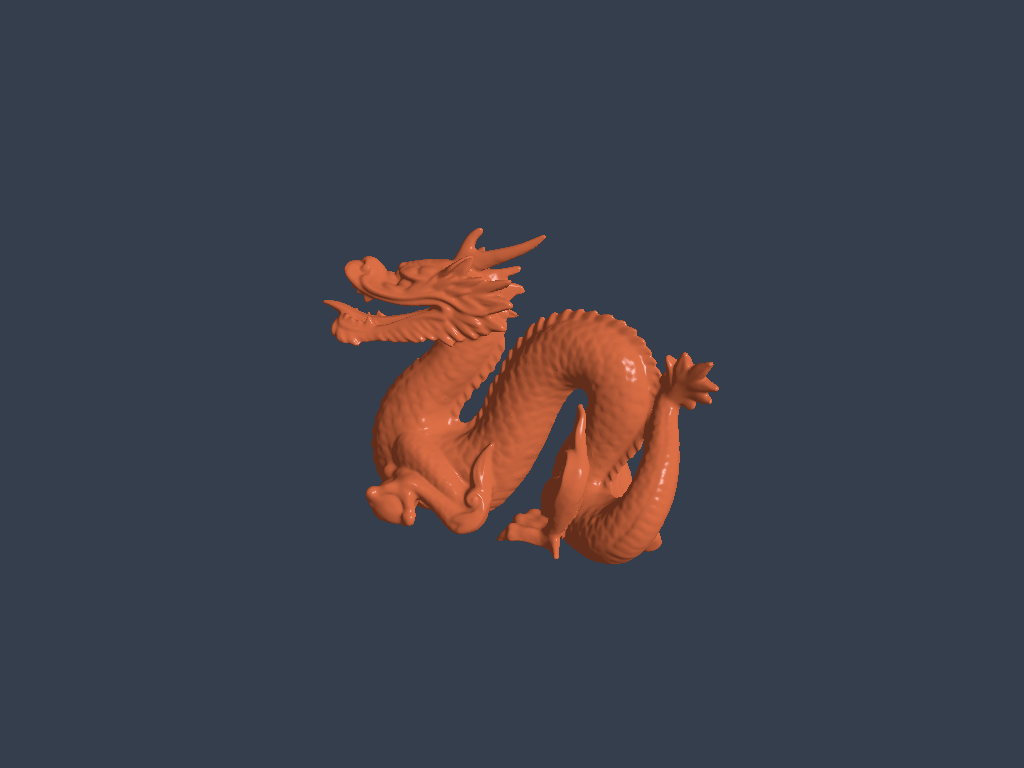
\includegraphics[width=0.5\linewidth]{imgs/hw_2_7.png}
    \caption{Reference rendering for homework 2.7.}
    \label{fig:hw2_7}
\end{figure}

\section{Make your own scene (5 points)}

As usual, design a scene yourself and submit the scene and your rendering to us. Feel free to download 3D model files on the internet (please credit the authors and let us know where you downloaded it). Note that our scene/mesh format may not be fully compatible with what you downloaded.
Please also submit all mesh and texture files referenced by your scene, so that we can reproduce your rendering.

\end{document}